% Options for packages loaded elsewhere
\PassOptionsToPackage{unicode}{hyperref}
\PassOptionsToPackage{hyphens}{url}
\PassOptionsToPackage{dvipsnames,svgnames,x11names}{xcolor}
\documentclass[
  10pt,
  fontset=fandol]{ctexart}
\usepackage{xcolor}
\usepackage[margin=16mm]{geometry}
\usepackage{amsmath,amssymb}
\setcounter{secnumdepth}{-\maxdimen} % remove section numbering
\usepackage{iftex}
\ifPDFTeX
  \usepackage[T1]{fontenc}
  \usepackage[utf8]{inputenc}
  \usepackage{textcomp} % provide euro and other symbols
\else % if luatex or xetex
  \usepackage{unicode-math} % this also loads fontspec
  \defaultfontfeatures{Scale=MatchLowercase}
  \defaultfontfeatures[\rmfamily]{Ligatures=TeX,Scale=1}
\fi
\usepackage{lmodern}
\ifPDFTeX\else
  % xetex/luatex font selection
\fi
% Use upquote if available, for straight quotes in verbatim environments
\IfFileExists{upquote.sty}{\usepackage{upquote}}{}
\IfFileExists{microtype.sty}{% use microtype if available
  \usepackage[]{microtype}
  \UseMicrotypeSet[protrusion]{basicmath} % disable protrusion for tt fonts
}{}
\makeatletter
\@ifundefined{KOMAClassName}{% if non-KOMA class
  \IfFileExists{parskip.sty}{%
    \usepackage{parskip}
  }{% else
    \setlength{\parindent}{0pt}
    \setlength{\parskip}{6pt plus 2pt minus 1pt}}
}{% if KOMA class
  \KOMAoptions{parskip=half}}
\makeatother
\usepackage{graphicx}
\makeatletter
\newsavebox\pandoc@box
\newcommand*\pandocbounded[1]{% scales image to fit in text height/width
  \sbox\pandoc@box{#1}%
  \Gscale@div\@tempa{\textheight}{\dimexpr\ht\pandoc@box+\dp\pandoc@box\relax}%
  \Gscale@div\@tempb{\linewidth}{\wd\pandoc@box}%
  \ifdim\@tempb\p@<\@tempa\p@\let\@tempa\@tempb\fi% select the smaller of both
  \ifdim\@tempa\p@<\p@\scalebox{\@tempa}{\usebox\pandoc@box}%
  \else\usebox{\pandoc@box}%
  \fi%
}
% Set default figure placement to htbp
\def\fps@figure{htbp}
\makeatother
\setlength{\emergencystretch}{3em} % prevent overfull lines
\providecommand{\tightlist}{%
  \setlength{\itemsep}{0pt}\setlength{\parskip}{0pt}}
\usepackage{amsmath,amssymb,mathtools,needspace}
\xeCJKDeclareCharClass{CJK}{"2032,"0400->"04FF,"2160->"216B,"2460->"2473,"25A0,"25C7,"25CB,"25CF}
\IfFontExistsTF{Arial Unicode MS}{\xeCJKsetup{AutoFallBack=true}\setCJKfallbackfamilyfont{\CJKrmdefault}{Arial Unicode MS}}{}
\setcounter{secnumdepth}{0}
\setlength{\emergencystretch}{2em}
\allowdisplaybreaks
\usepackage{bookmark}
\IfFileExists{xurl.sty}{\usepackage{xurl}}{} % add URL line breaks if available
\urlstyle{same}
\hypersetup{
  pdftitle={引言与预备知识},
  colorlinks=true,
  linkcolor={Maroon},
  filecolor={Maroon},
  citecolor={Blue},
  urlcolor={Blue},
  pdfcreator={LaTeX via pandoc}}

\title{引言与预备知识}
\author{}
\date{}

\begin{document}
\maketitle

\subsection{3.1 引言与预备知识}\label{ux5f15ux8a00ux4e0eux9884ux5907ux77e5ux8bc6}

\subsubsection{3.1.1 问题的提出}\label{ux95eeux9898ux7684ux63d0ux51fa}

在数值计算中经常遇到求函数值的问题. 用手工计算时常常通过函数表求得; 用计算机计算时, 若把函数表存入内存进行查表, 则占用单元太多, 不如直接用公式计算方便. 因此, 我们希望求出便于计算且计算量省的公式近似已知函数 \(f(x)\). 例如, Taylor 展开式的部分和

\[
P_n(x) = f(x_0) + \frac{f'(x_0)}{1!}(x-x_0) + \cdots + \frac{f^{(n)}(x_0)}{n!}(x-x_0)^n \tag{3.1.1}
\]

就是 \(f(x)\)的一种近似公式. 用它求 \(x_0\) 附近的函数值 \(f(x)\) 误差较小, 当 \(|x-x_0|\) 较大时误差就很大. 例如 \(f(x)=e^x\) 在 \([-1,1]\) 上用

\[
P_4(x) = 1+x+\frac{1}{2}x^2+\frac{1}{6}x^3+\frac{1}{24}x^4
\]

近似 \(e^x\), 其误差

\[
R_4(x)=e^x-P_4(x)=\frac{1}{120}x^5e^\epsilon, \quad \epsilon \in(-1,1),
\]

于是

\[
|R_4(x)| \leqslant \frac{e}{120}|x^5|, \quad \max_{-1 \leqslant x \leqslant 1}|R_4(x)| \leqslant \frac{e}{120} \approx 0.0226.
\]

误差分布如图3.1所示, 它在整个区间上误差较大. 若在计算机上用这种方法计算 \(e^x\), 如精度要求较高, 则需取很多项, 这样既费时又多占存储单元, 因此, 要求在给定精度下求计算次数最少的近似公式, 这就是函数逼近与计算要解决的问题. 这问题可叙述为: ``对于函数类 \(A\) 中给定的函数 \(f(x)\), 要求在另一类较简单的便于计算的函数类 \(B\) 中, 求函数 \(P(x) \in B \subseteq A\), 使 \(P(x)\) 与 \(f(x)\) 之差在某种度量意义下最小.'' 函数类 \(A\) 通常是区间 \([a,b]\) 上的连续函数, 记作 \(C[a,b]\); 函数类 \(B\) 通常是代数多项式、分式有理函数或三角多项式. 而度量标准最常用的有两种,一种是

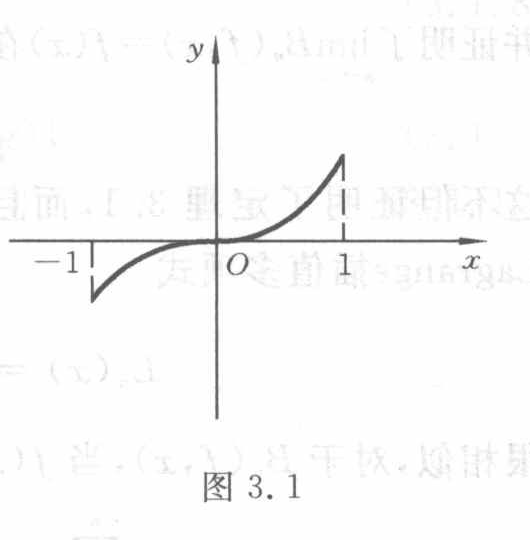
\includegraphics[width=0.85\linewidth,height=\textheight,keepaspectratio,alt={图 3.1 原图裁切}]{../assets/ch03a/fig-3-1.png}

图 3.1（原图）。图中为上文误差分布曲线，横轴 \(x\)、纵轴 \(y\)；标签为 \(-1\)、\(1\)、\(O\)。曲线在负半轴下方、正半轴上方，通过原点；在 \(x=-1\) 和 \(x=1\) 处有竖向辅助线。

\href{../../source-images/pdf-059.jpeg}{查看原页}

\[
\| f(x) - P(x) \|_{\infty} = \max_{a \leqslant x \leqslant b} |f(x) - P(x)|, \tag{3.1.2}
\]

在这种度量意义下的函数逼近称为一致逼近或均匀逼近；另一种度量标准是 \[
\| f(x) - P(x) \|_{2} = \sqrt{\int_{a}^{b} [f(x) - P(x)]^{2} \mathrm{d}x}, \tag{3.1.3}
\]

用这种度量的函数逼近称为均方逼近或平方逼近. 这里, 符号 \(\| \cdot \|_{\infty}\) 及 \(\| \cdot \|_{2}\) 是范数. 本章主要研究在这两种度量标准下用代数多项式 \(P_{n}(x)\) 逼近 \(f(x) \in C[a,b]\), 也就是用最佳一致逼近多项式与最佳平方逼近多项式逼近 \(f(x) \in C[a,b]\).

\subsubsection{3.1.2 Weierstrass 定理}\label{weierstrass-ux5b9aux7406}

用插值法或 Taylor 展开求 \(f(x) \in C[a,b]\) 的逼近多项式, 在某些点上可能没有误差, 但在整个区间 \([a,b]\) 上误差可能很大, 2.7 节给出的 Runge 现象就说明了这一点. 因此, 用 \(P_{n}(x)\) 一致逼近 \(f(x)\), 首先要解决存在性问题, 即对于 \([a,b]\) 上的连续函数 \(f(x)\), 是否存在多项式 \(P_{n}(x)\) 一致收敛于 \(f(x)\)? Weierstrass 给出了下面定理.

定理 3.1 设 \(f(x) \in C[a,b]\), 则对于任何 \(\varepsilon > 0\), 总存在一个代数多项式 \(P(x)\), 使 \[
\| f(x) - P(x) \|_{\infty} < \varepsilon
\] 在 \([a,b]\) 上一致成立.

这定理已在``数学分析''中证明过. 这里需要说明的是在许多证明方法中, Bernstein 在 1912 年给出的证明是一种构造性证明. 他根据函数整体逼近的特性造出 Bernstein 多项式 \[
\begin{cases} B_{n}(f,x) = \sum_{k=0}^{n} f\left(\frac{k}{n}\right) P_{k}(x), \\ P_{k}(x) = \binom{n}{k} x^{k}(1-x)^{n-k}, \end{cases} \tag{3.1.4}
\]

并证明了 \(\lim_{n \to \infty} B_{n}(f,x) = f(x)\) 在 \([0,1]\) 上一致成立; 若 \(f(x)\) 在 \([0,1]\) 上 \(m\) 阶导数连续, 则 \[
\lim_{n \to \infty} B_{n}^{(m)}(f,x) = f^{(m)}(x).
\] 这不但证明了定理 3.1, 而且由式 (3.1.4)给出了 \(f(x)\) 的一个逼近多项式. 它与 Lagrange 插值多项式 \[
L_{n}(x) = \sum_{k=0}^{n} f\left(x_{k}\right) l_{k}(x), \quad \sum_{k=0}^{n} l_{k}(x_{k}) = 1
\] 很相似, 对于 \(B_{n}(f,x)\), 当 \(f(x)=1\) 时也有关系式 \[
\sum_{k=0}^{n} P_{k}(x) = \sum_{k=0}^{n} \binom{n}{k} x^{k}(1-x)^{n-k} = 1. \tag{3.1.5}
\]

这只要从恒等式

\begin{quote}
校注（agent 补充，原书疑误）：原页 Lagrange 插值式后的求和明确印为 \(\sum_{k=0}^{n}l_k(x_k)=1\)，此处按原文保留。由基函数性质 \(l_k(x_k)=1\)，左端应为 \(n+1\)；通常的恒等式应为 \(\sum_{k=0}^{n}l_k(x)=1\)。这不是 OCR 误识。
\end{quote}

\href{../../source-images/pdf-060.jpeg}{查看原页}

\[
(x+y)^n = \sum_{k=0}^{n} \binom{n}{k} x^k y^{n-k} \tag{3.1.6}
\] 中令 \(y=1-x\) 就可得到. 但这里当 \(x \in [0,1]\) 时还有 \(P_k(x) \geqslant 0\), 于是 \[
\sum_{k=0}^{n} |P_k(x)| = \sum_{k=0}^{n} P_k(x) = 1
\] 是有界的, 因而只要 \(|f(x)| \leqslant \delta\) 对于任意 \(x \in [0,1]\) 成立, 则 \[
|B_n(f,x)| \leqslant \max_{0 \leqslant x \leqslant 1} |f(x)| \sum_{k=0}^{n} |P_k(x)| \leqslant \delta
\] 有界, 故 \(B_n(f,x)\) 是稳定的. 至于 Lagrange 插值多项式 \(L_n(x)\), 由于 \(\sum_{k=0}^{n} |l_k(x)|\) 无界, 因而不能保证高阶插值的稳定性与收敛性. 相比之下, 多项式 \(B_n(f,x)\) 有良好的逼近性质, 但它收敛太慢, 比三次样条逼近效果差得多, 实际中很少使用.

\subsubsection{\texorpdfstring{3.1.3 连续函数空间 \(C[a,b]\)}{3.1.3 连续函数空间 C{[}a,b{]}}}\label{ux8fdeux7eedux51fdux6570ux7a7aux95f4-cab}

区间 \([a,b]\) 上的所有实连续函数组成一个空间, 记作 \(C[a,b]\). \(f \in C[a,b]\) 的范数定义为 \[
\|f\|_\infty = \max_{a \leqslant x \leqslant b} |f(x)| ,
\] \(\|\cdot\|_\infty\) 称为 \(\infty\)-范数, 它满足范数 \(\|\cdot\|\) 的三个性质: (1) \(\|f\| \geqslant 0\), 当且仅当 \(f \equiv 0\) 时才有 \(\|f\| = 0\); (2) \(\|af\| = |a| \|f\|\) 对于任意 \(f \in C[a,b]\) 成立, \(a\) 为任意实数; (3) 对于任意 \(f,g \in C[a,b]\), 有 \[
\|f+g\| \leqslant \|f\| + \|g\| \tag{3.1.7}
\] 式(3.1.7)称为三角不等式. 空间 \(C[a,b]\) 可与向量空间类比, 函数 \(f \in C[a,b]\) 可看成向量. 与向量空间类似, 当 \(f,g \in C[a,b]\) 时, 定义 \(f\) 与 \(g\) 的距离为 \[
D(f,g) = \|f-g\|_\infty \tag{3.1.8}
\] 由式(3.1.7)可得到 \[
D(f,g) \leqslant D(f,h) + D(h,g) \tag{3.1.9}
\] \[
\bigl|\|f\|_\infty - \|g\|_\infty\bigr| \leqslant \|f-g\|_\infty \tag{3.1.10}
\]

\subsection{本节覆盖原页的校注记录}\label{ux672cux8282ux8986ux76d6ux539fux9875ux7684ux6821ux6ce8ux8bb0ux5f55}

下列记录按原页关联，含同页相邻小节的校注；计算时同时读取上文校注和完整原页。

\begin{itemize}
\tightlist
\item
  \texttt{ch03a-E01}：原书 PDF 页 59
\end{itemize}

\end{document}
